\documentclass{beamer}
\usepackage[german,english]{babel}
\usepackage[utf8x]{inputenc}

\usepackage{graphicx}
\usepackage{svg}
\usepackage{wrapfig}
\usepackage{eurosym}
\usepackage{tabularx}
\usepackage{multirow}

\usepackage{listings}
\usepackage{color}

\definecolor{codegreen}{rgb}{0,0.6,0}
\definecolor{codegray}{rgb}{0.5,0.5,0.5}
\definecolor{codepurple}{rgb}{0.58,0,0.82}
\definecolor{backcolour}{rgb}{1.0,1.0,1.0}

\lstdefinestyle{mystyle}{
	backgroundcolor=\color{backcolour},   
	commentstyle=\color{codegreen},
	keywordstyle=\color{magenta},
	numberstyle=\tiny\color{codegray},
	stringstyle=\color{codepurple},
	basicstyle=\footnotesize,
	breakatwhitespace=false,         
	breaklines=true,                 
	captionpos=b,                    
	keepspaces=true,                 
	numbers=left,                    
	numbersep=5pt,                  
	showspaces=false,                
	showstringspaces=false,
	showtabs=false,                  
	tabsize=2
}

\lstset{style=mystyle}

\usetheme{CambridgeUS}
% Other valid themes
%   Antibes, Bergen, Berkeley, Berlin, Copenhagen
%   Darmstadt, Dresden, Frankfurt, Goettingen, Hannover
%   Ilmenau, JuanLesPins, Luebeck, Madrid, Malmoe
%   Marburg, Montpellier, PaloAlto, Pittsburgh, Rochester
%   Singapore, Szeged, Warsaw, boxes, default

\usecolortheme{default}
% Other valid color schemes
%    albatross, beaver, beetle, crane, dolphin
%    dove, fly, lily, orchid, rose, seagull
%    seahorse, whale and the one and only wolverine

\title[Project 1]{Project 1}
\subtitle{Pytho Intro}
\author{}
\institute[Universität Bonn]{Rheinische Friedrich-Wilhelms-Universität}
\date{\today}

\begin{document}
	
\begin{frame}%1
	\titlepage
\end{frame}

\begin{frame}%2
\frametitle{Table of Contents}
\tableofcontents%[pausesections]
\end{frame}


\section{Task 1.1}

\begin{frame}[fragile]
\frametitle{Filtering Outliers}

\begin{lstlisting}[language=Python]
	data = data[np.all(data[:,0:2].astype(float)>0,axis=1)]
\end{lstlisting}
\end{frame}

\begin{frame}
\frametitle{Plots}
With outliers on the left. No outliers on the right.
\begin{figure}
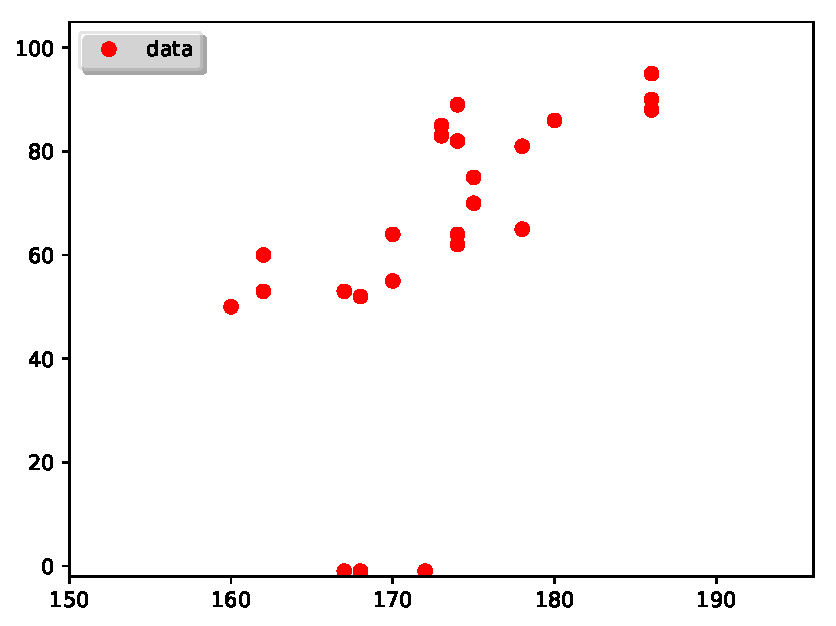
\includegraphics[width=0.475\textwidth]{graphics/plotHW}
\hfill
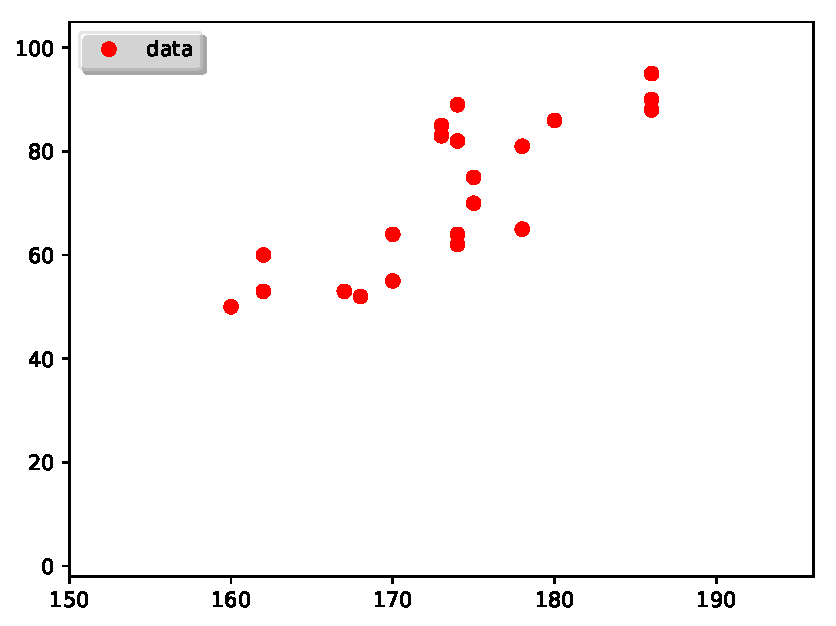
\includegraphics[width=0.475\textwidth]{graphics/plotHW_no_outlier}
\end{figure}
\end{frame}


\begin{frame}
\frametitle{}
\begin{itemize}
\item<1-> point 1
\item<1-> point 2
\item<1-> point 3
\end{itemize}
\end{frame}

\section{Task 1.2}
\section{Task 1.3}
\section{Task 1.4}
\section{Task 1.5}

\begin{frame}
\begin{center}
\LARGE
Thank you for your attention!
\begin{center}
\LARGE
Questions?
\end{center}
\end{center}
\end{frame}



%\bibliography{Bibliography}
%\bibliographystyle{plain}

%\begin{thebibliography}{}
%\bibitem{1} 
%\bibitem{2} 
%\bibitem{3} 
%\end{thebibliography}


\end{document} 
